\documentclass[journal,12pt,twocolumn]{IEEEtran}

\usepackage{setspace}
\usepackage{gensymb}
\singlespacing
\usepackage[cmex10]{amsmath}
\usepackage{cancel}
\usepackage{amsthm}
\usepackage{amsmath}
\usepackage{paralist}
\usepackage{upgreek}
\usepackage{mathrsfs}
\usepackage{txfonts}
\usepackage{stfloats}
\usepackage{bm}
\usepackage{cite}
\usepackage{cases}
\usepackage{subfig}

\usepackage{longtable}
\usepackage{multirow}
\usepackage{enumitem}
\usepackage{mathtools}
\usepackage{steinmetz}
\usepackage{tikz}
\usepackage{circuitikz}
\usepackage{verbatim}
\usepackage{tfrupee}
\usepackage[breaklinks=true]{hyperref}
\usepackage{graphicx}
\usepackage{tkz-euclide}

\usetikzlibrary{calc,math}
\usepackage{listings}
    \usepackage{color}                                            %%
    \usepackage{array}                                            %%
    \usepackage{longtable}                                        %%
    \usepackage{calc}                                             %%
    \usepackage{multirow}                                         %%
    \usepackage{hhline}                                           %%
    \usepackage{ifthen}                                           %%
    \usepackage{lscape}     
\usepackage{multicol}
\usepackage{chngcntr}

\DeclareMathOperator*{\Res}{Res}
\usepackage{romannum}
\renewcommand\thesection{\arabic{section}}
\renewcommand\thesubsection{\thesection.\arabic{subsection}}
\renewcommand\thesubsubsection{\thesubsection.\arabic{subsubsection}}

\renewcommand\thesectiondis{\arabic{section}}
\renewcommand\thesubsectiondis{\thesectiondis.\arabic{subsection}}
\renewcommand\thesubsubsectiondis{\thesubsectiondis.\arabic{sub subsection}}


\hyphenation{optical networks semiconduc-tor}
\def\inputGnumericTable{}                                 %%

\lstset{
%language=C,
frame=single, 
breaklines=true,
columns=fullflexible
}
\date{March 2021}

\begin{document}
\newcommand{\multlinecomment}[1]{\directlua{-- #1}}
\newcommand{\BEQA}{\begin{eqnarray}}
\newcommand{\EEQA}{\end{eqnarray}}
\newcommand{\define}{\stackrel{\triangle}{=}}
\bibliographystyle{IEEEtran}
\raggedbottom
\setlength{\parindent}{0pt}
\providecommand{\mbf}{\mathbf}
\providecommand{\pr}[1]{\ensuremath{\Pr\left(#1\right)}}
\providecommand{\qfunc}[1]{\ensuremath{Q\left(#1\right)}}
\providecommand{\fn}[1]{\ensuremath{f\left(#1\right)}}
\providecommand{\e}[1]{\ensuremath{E\left(#1\right)}}
\providecommand{\sbrak}[1]{\ensuremath{{}\left[#1\right]}}
\providecommand{\lsbrak}[1]{\ensuremath{{}\left[#1\right.}}
\providecommand{\rsbrak}[1]{\ensuremath{{}\left.#1\right]}}
\providecommand{\brak}[1]{\ensuremath{\left(#1\right)}}
\providecommand{\lbrak}[1]{\ensuremath{\left(#1\right.}}
\providecommand{\rbrak}[1]{\ensuremath{\left.#1\right)}}
\providecommand{\cbrak}[1]{\ensuremath{\left\{#1\right\}}}
\providecommand{\lcbrak}[1]{\ensuremath{\left\{#1\right.}}
\providecommand{\rcbrak}[1]{\ensuremath{\left.#1\right\}}}
\theoremstyle{remark}
\newtheorem{rem}{Remark}
\newcommand{\sgn}{\mathop{\mathrm{sgn}}}
\providecommand{\abs}[1]{\vert#1\vert}
\providecommand{\res}[1]{\Res\displaylimits_{#1}} 
\providecommand{\norm}[1]{\lVert#1\rVert}
%\providecommand{\norm}[1]{\lVert#1\rVert}
\providecommand{\mtx}[1]{\mathbf{#1}}
\providecommand{\mean}[1]{E[ #1 ]}
\providecommand{\fourier}{\overset{\mathcal{F}}{ \rightleftharpoons}}
%\providecommand{\hilbert}{\overset{\mathcal{H}}{ \rightleftharpoons}}
\providecommand{\system}{\overset{\mathcal{H}}{ \longleftrightarrow}}
	%\newcommand{\solution}[2]{\textbf{Solution:}{#1}}
\newcommand{\solution}{\noindent \textbf{Solution: }}
\newcommand{\cosec}{\,\text{cosec}\,}
\providecommand{\dec}[2]{\ensuremath{\overset{#1}{\underset{#2}{\gtrless}}}}
\newcommand{\myvec}[1]{\ensuremath{\begin{pmatrix}#1\end{pmatrix}}}
\newcommand{\mydet}[1]{\ensuremath{\begin{vmatrix}#1\end{vmatrix}}}
\numberwithin{equation}{subsection}
\makeatletter
\vspace{3cm}
\title{Gate Assignment 4}
\author{RONGALA ARUN SIDDARDHA - AI20BTECH11019}
\maketitle
\newpage
\bigskip
\renewcommand{\thetable}{\theenumi}

%
Download latex code from 
%
\begin{lstlisting}
https://github.com/ArunSiddardha/EE900/tree/main/Gate_assignment/Gate_Assignment.tex
\end{lstlisting}

\section*{GATE-EC 1997 Q.1.5}
The Laplace Transform of $e^{a t}cos(a t)$ 
\begin{enumerate}
    \item $\frac{s-a}{(s - a)^2 + a^2}$\\
  \item $\frac{s+a}{(s - a)^2 + a^2}$\\
  \item $\frac{1}{(s - a)^2}$\\
  \item None of these
\end{enumerate}
\section*{Solution}
let h(t) = $e^{a t}cos(a t)$  \\ 
\begin{align}
    h(t)&=e^{a t}cos(a t)\\
        &= e^{a t}\brak{\frac{e^{i a t} + e^{-i a t}}{2}}\\
        &=\frac{e^{(i+1) a t} + e^{(1-i) a t}}{2}
\end{align}
Taking one-sided Laplace transform for h(t)
\begin{align}
    \mathcal{L}\cbrak{h(t)}(s)= \frac{1}{2}\brak{\mathcal{L}\brak{e^{(i+1) a t}}(s)+\mathcal{L}\brak{e^{(i+1) a t}}(s)}\\
    \text{We know that, }
    \mathcal{L}\cbrak{e^{at}}(s)=\int^{\infty}_{0}e^{a t}e^{st}dt=\frac{1}{s-a} \\
    =\frac{1}{2}\brak{\frac{1}{s-(i+1)a}+ \frac{1}{s-(1-i)a}}\\
    =\frac{(s-a)}{(s-a)^2+a^2}
\end{align}
Answer is \textbf{option 1}\\\\\\
Zero is at $(a,0)$ and there are two complex poles at $a + ia$ and $a-ia$.
The ROC for this plot for the above function is given by 
\begin{align}
    \mathcal{R}e\cbrak{s}>\mathcal{R}e\cbrak{a}
\end{align}

\begin{figure}[htp]
    \centering
    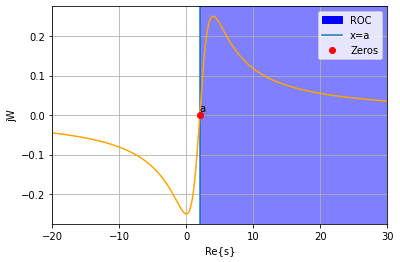
\includegraphics[width = \columnwidth]{fig.png}
    \caption{ROC plot}
    \label{fig:my_label}
\end{figure}


\end{document}

